%\documentclass{beamer}
%\documentclass[c]{beamer}
 \documentclass[t]{beamer}
%\documentclass[b]{beamer}
\listfiles

\mode<presentation>
{
  \usetheme[english]{KIT}
% \usetheme[usefoot]{KIT}
% \usetheme[deutsch]{KIT}

%%  \usefonttheme{structurebold}

  \setbeamercovered{transparent}

  %\setbeamertemplate{enumerate items}[circle]
  \setbeamertemplate{enumerate items}[ball]
}

\usepackage{babel}
\date{03.10.13}
%\DateText

%\KITfoot{\parbox[t]{90mm}{\today:\qquad Dies ist eine sehr lange selbstdefinierte Fu\ss{}zeile -- Dies ist eine sehr lange selbstdefinierte Fu\ss{}zeile -- Dies ist eine sehr lange selbstdefinierte Fu\ss{}zeile}}


\usepackage[utf8]{inputenc}
\usepackage[T2A]{fontenc}
\usepackage{array}
\usepackage{minted}

\usenavigationsymbols
%\usenavigationsymbols[sfHhdb]
%\usenavigationsymbols[sfhHb]

%\title[Python Interfaces for reactor codes]{Python Interfaces for Reactor Codes}
\title[Python-интерфейсы для программ расчета реакторов]{PIRS: Интерфейсы языка программирования Python для программ расчета реакторов}
\subtitle{Безопасность АЭС и подготовка кадров, Обнинск-2013}

%\author{A.Travleev, R. Molitor, V.H. Sanchez}
\author{А. Травлеев, Р. Молитор, В. Санчез}

%\institute{Карлсруйский технологический институт, институт физики нейтронов и техники реакторов}
\institute{Institute for Neutron Physics and Reactor Technology}

%\TitleImage[height=\titleimageht]{Bilder/bildwand.jpg}
\TitleImage[height=\titleimageht]{Bilder/KIT-Titel.png}


\begin{document}

\begin{frame}
  \maketitle
\end{frame}

\begin{frame}\frametitle{Содержание}

    \begin{itemize}
        \item Введение: определения и пример

        \item Концепция

        \item текущий статус разработки

        \item что впереди

    \end{itemize}
\end{frame}

\section{Введение}
\begin{frame}\frametitle{Что это?}

    \begin{block}{PIRS: Python Interfaces for Reactor Simulations}

    Набор пакетов для языка программирования Питон, которые облегчают 
    взаимодействие пользователя с программами расчета реакторов.
    \end{block}

    \begin{columns}
        \column{0.45\textwidth}
    \begin{block}{Python}
    \begin{itemize}

        \item www.python.org

        \item свободно распространяемый

        \item интерпретируемый

        \item ОС-независимый

        \item большая группа пользователей

        \item широкий спектр пакетов

    \end{itemize}
    \end{block}

        \column{0.45\textwidth}
    \begin{block}{Взаимодействие}
    \begin{itemize}
        
        \item описание модели

        \item подготовка инпута

        \item запуск программы расчета

        \item  чтение результатов расчета

    \end{itemize}
    \end{block}
    \end{columns}
\end{frame}

\begin{frame}\frametitle{Для чего PIRS  нужен?}    

    
    \begin{itemize}
    \item Рутинная подготовка интпутов 

    \item Организация совместных итерационных расчетов

    \item ...
    \end{itemize}

\end{frame}

\begin{frame}[fragile]
    \frametitle{Пример: упрощенная нейтронно-физическая модель ТВЭЛа}

    Описание геометрии
    \inputminted[frame=single,fontfamily=tt,fontsize=\footnotesize]{python}{geom.py}

\end{frame}

\begin{frame}[fragile]
    \frametitle{Пример: упрощенная нейтронно-физическая модель ТВЭЛа}

    Описание нейтронно-физических характеристик

    \begin{columns}
        \column{0.45\textwidth}
            \inputminted[frame=single,fontfamily=tt,fontsize=\footnotesize,firstline=3,lastline=17]{python}{mc_int.py}
        \column{0.45\textwidth}
            \inputminted[frame=single,fontfamily=tt,fontsize=\footnotesize,firstline=17]{python}{mc_int.py}
    \end{columns}

\end{frame}

\begin{frame}[fragile]
    \frametitle{Пример: упрощенная нейтронно-физическая модель ТВЭЛа}
    \begin{columns}
        \column{0.45\textwidth}
            \inputminted[frame=single,fontfamily=tt,fontsize=\tiny,firstline=3,lastline=30]{rst}{mcnp0/i_}
        \column{0.45\textwidth}
            \inputminted[frame=single,fontfamily=tt,fontsize=\tiny,firstline=31]{rst}{mcnp0/i_}
    \end{columns}
\end{frame}

\begin{frame}[fragile]
    \frametitle{Пример: упрощенная нейтронно-физическая модель ТВЭЛа}


            \includegraphics[width=0.7\textwidth]{mcnp0/i__p02.pdf}
\end{frame}

\section{Концепция}
\begin{frame}\frametitle{Концепция}
    \begin{block}{Типы классов}
        \begin{itemize}
            \item Для описания расчетной геометрии:
                  Базовые объемы (цилиндр, бокс), которые можно вставлять друг
                  в друга и задавать положение.

            \item Интерфейсы низкого уровня:
                  Правильность синтаксиса входного файла, процедуры для чтения
                  результатов расчета, правила запуска расчетных програм.

            \item Интерфейсы высокого уровня:
                  Конвертация геометрии в инпут и результатов обратно в
                  геометрию, определение параметров, специфических для кода
                  (путь файлам данных для MCNP, например)
        \end{itemize}
    \end{block}

    \begin{block}{Типы пользователей}
        \begin{itemize}
            \item расчетчики: используют геометрические классы и классы высокого уровня
            \item разработчики интерфейсов: пишут интерфейсы
        \end{itemize}
    \end{block}
\end{frame}
\begin{frame}\frametitle{Взаимодействие классов}
   
   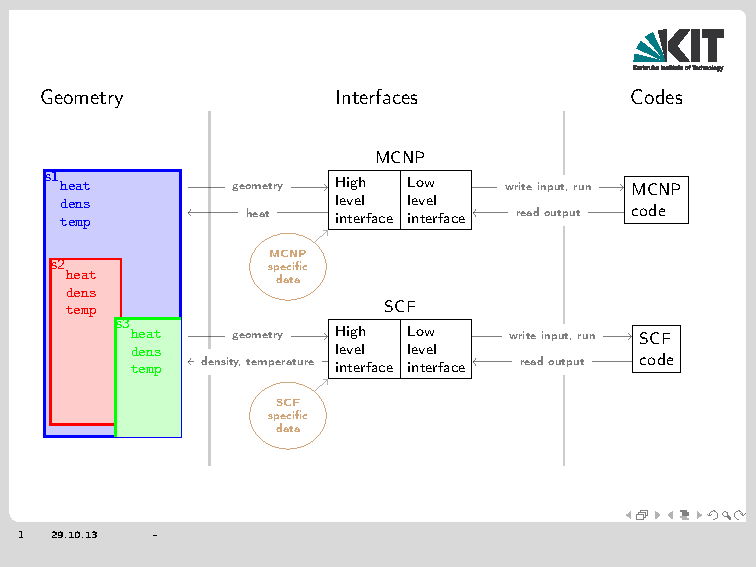
\includegraphics[trim=0 180 0 0,clip=true,width=0.7\textwidth]{pics/scheme.pdf}

\end{frame}

\section{Текущий статус разработки}
\begin{frame}\frametitle{Текущий статус разработки}
    Определен во многом целями проекта, в рамках которого PIRS разрабатывается: НФ и ТГ моделирование АЗ PWR.
    \begin{block}{Геометрия} 
        \begin{itemize}
            \item Cylinder: вертикальный цилиндр конечной высоты
            \item Box: прямоугольный параллелепипед со сторонами перпендикулярными к осям
        \end{itemize}
    \end{block}
    
    \begin{columns}
    \column{0.47\textwidth}
    \begin{block}{Интерфейс MCNP}
        \begin{itemize}
            \item для произвольной геометрии
            \item использование решетки (lattice card)
            \item описание материалов
            \item чтение meshtal
        \end{itemize}
    \end{block}

    \column{0.47\textwidth}
    \begin{block}{Интерфейс SCF}
        \begin{itemize}
            \item для геометрии ТВС
            \item чтение результатов из output.txt
        \end{itemize}
    \end{block}
    \end{columns}

\end{frame}


\begin{frame}\frametitle{Пример: результат совместного итеративного расчета}

    Модель: ТВС 17x17 с каналами для замедлителя и двумя типами ТВЭЛов.

    Совместный MCNP -- SCF расчет, организованный с помощью PIRS

    
    \begin{columns}
        \column{0.49\textwidth}
            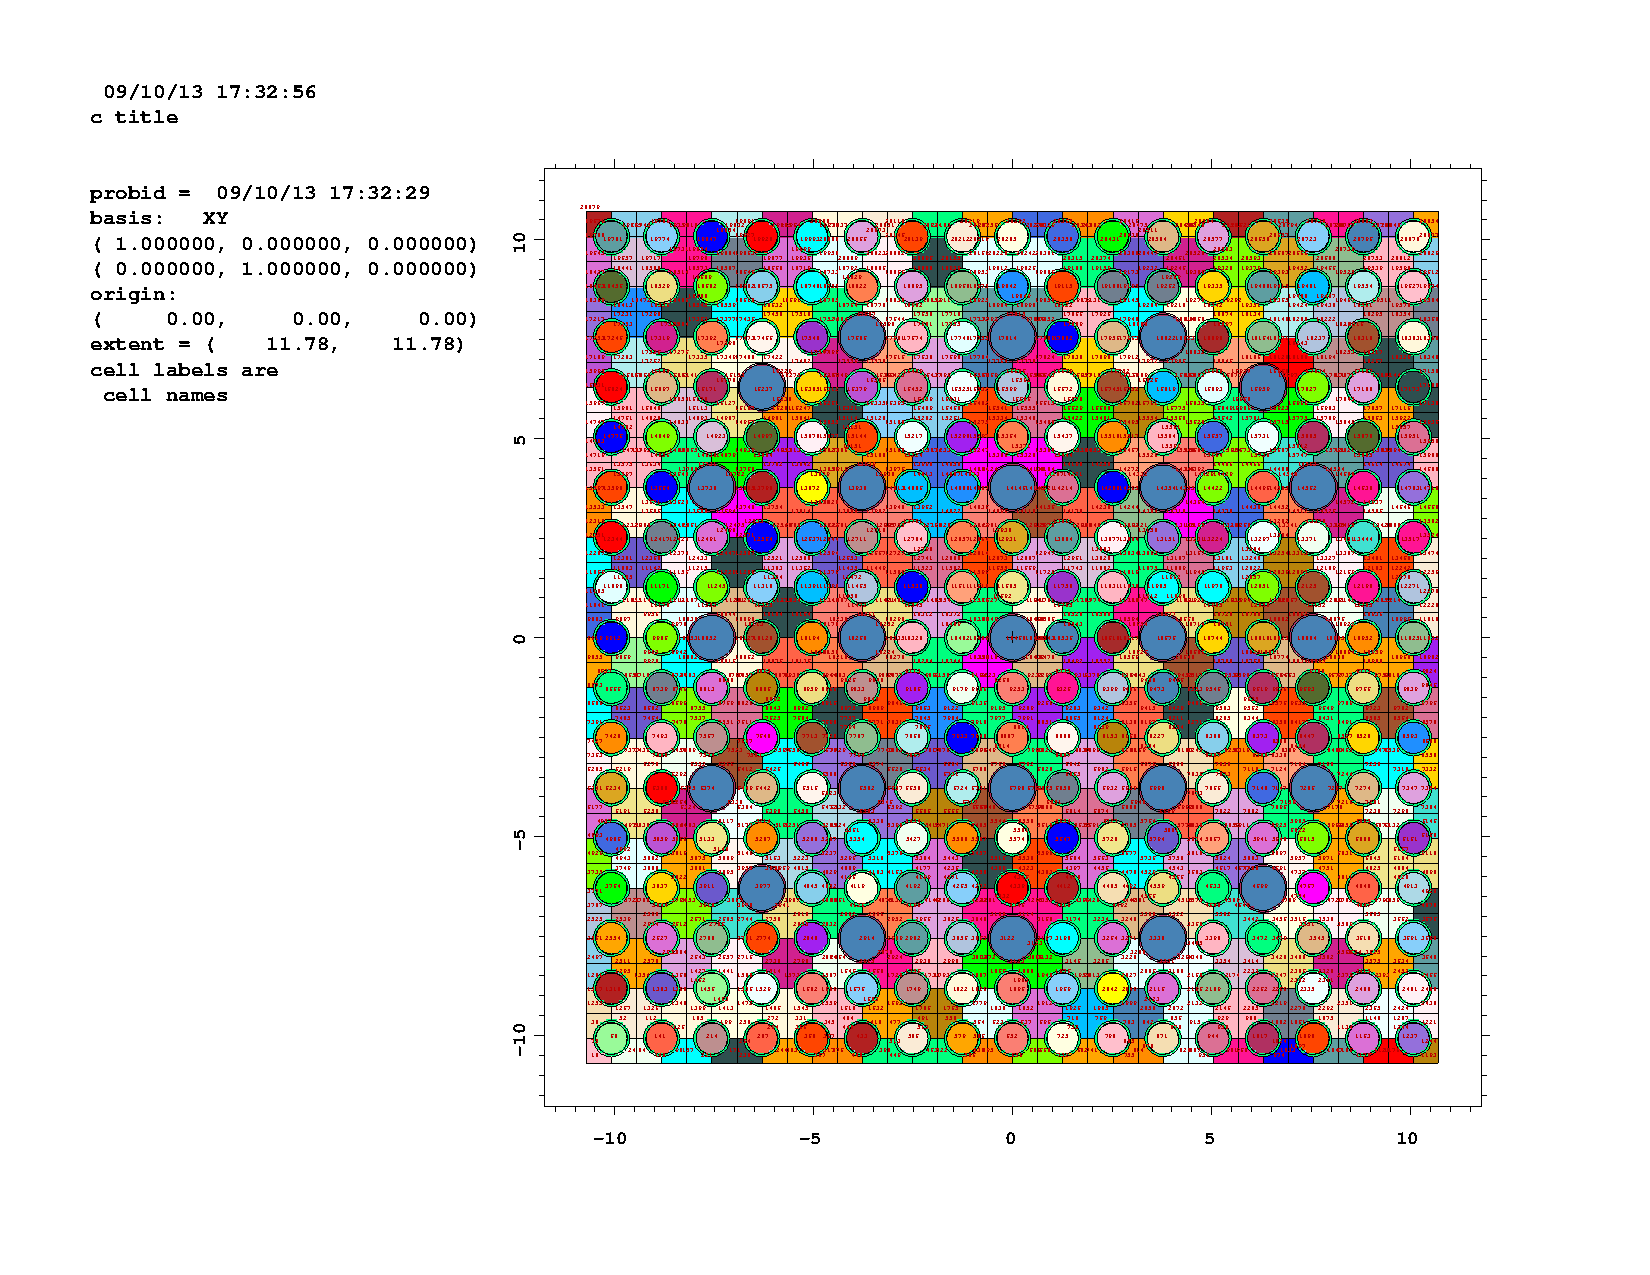
\includegraphics[width=1.2\textwidth]{pics/i__p01.pdf}
        \column{0.49\textwidth}
            \includegraphics[width=1.2\textwidth]{pics/i__p02.pdf}
    \end{columns}

\end{frame}

\begin{frame}\frametitle{Пример: результат совместного итеративного расчтеа}

    Изменение $k_{eff}$ с итерациями
    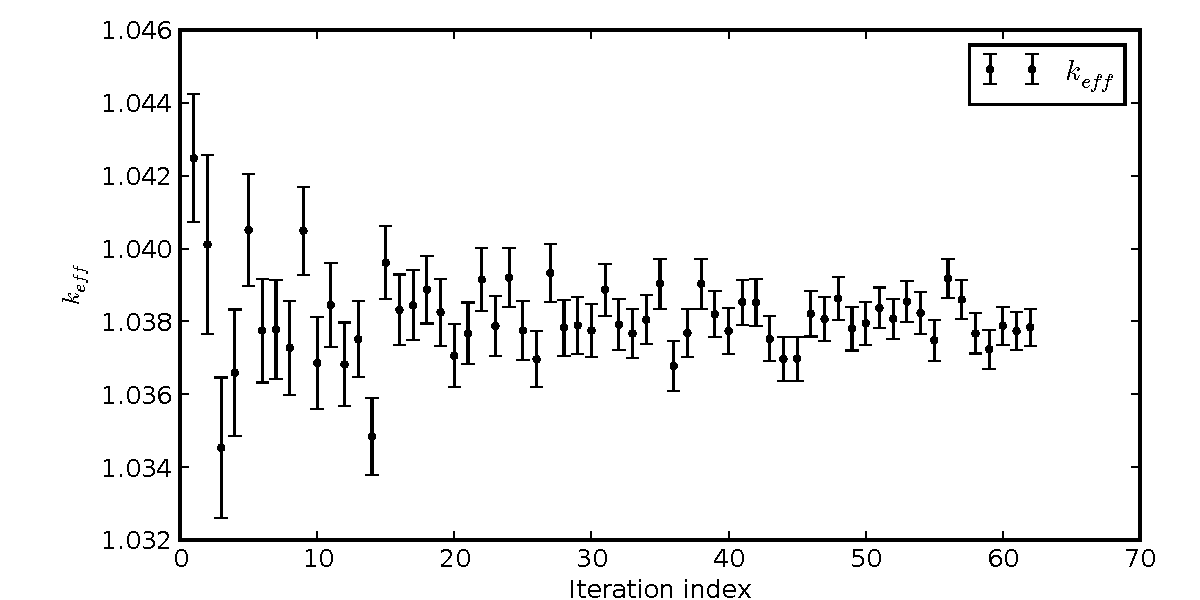
\includegraphics[width=0.8\textwidth]{pics/b_iteration_062_keff.pdf}
\end{frame}

\begin{frame}\frametitle{Пример: результат совместного итеративного расчтеа}
    Аксиальное распределение энерговыделения в одном из ТВЭЛов
    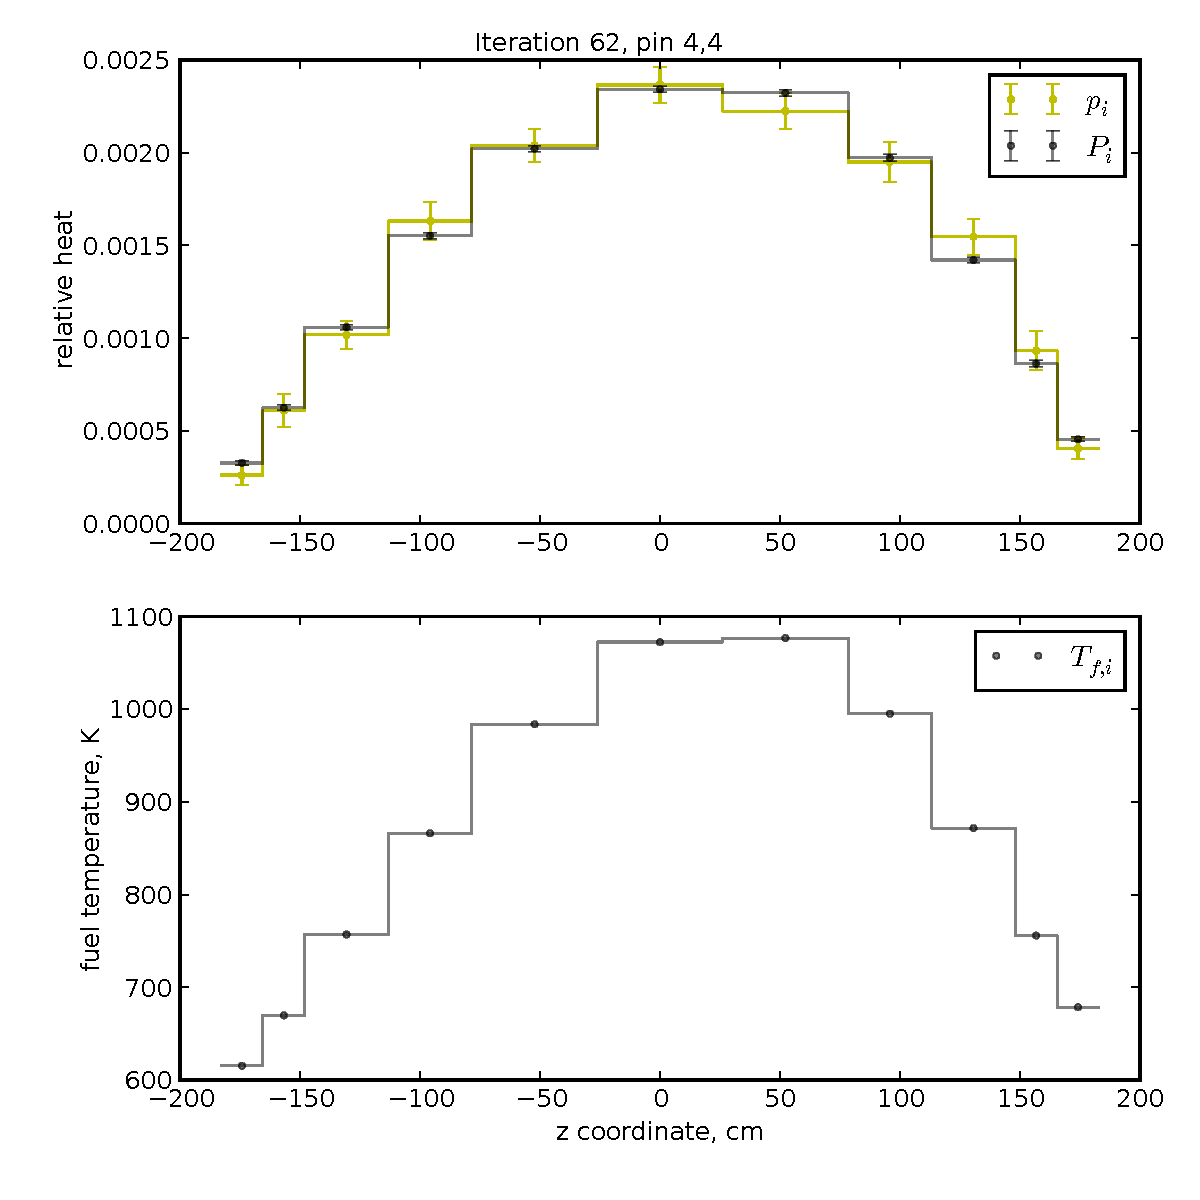
\includegraphics[trim=0 300 0 0,clip=true,width=0.8\textwidth]{pics/b_iteration_062_4_4.pdf}
\end{frame}

\begin{frame}\frametitle{Пример: результат совместного итеративного расчтеа}
    Аксиальное распределение температуры в топливе в том-же ТВЭЛе
    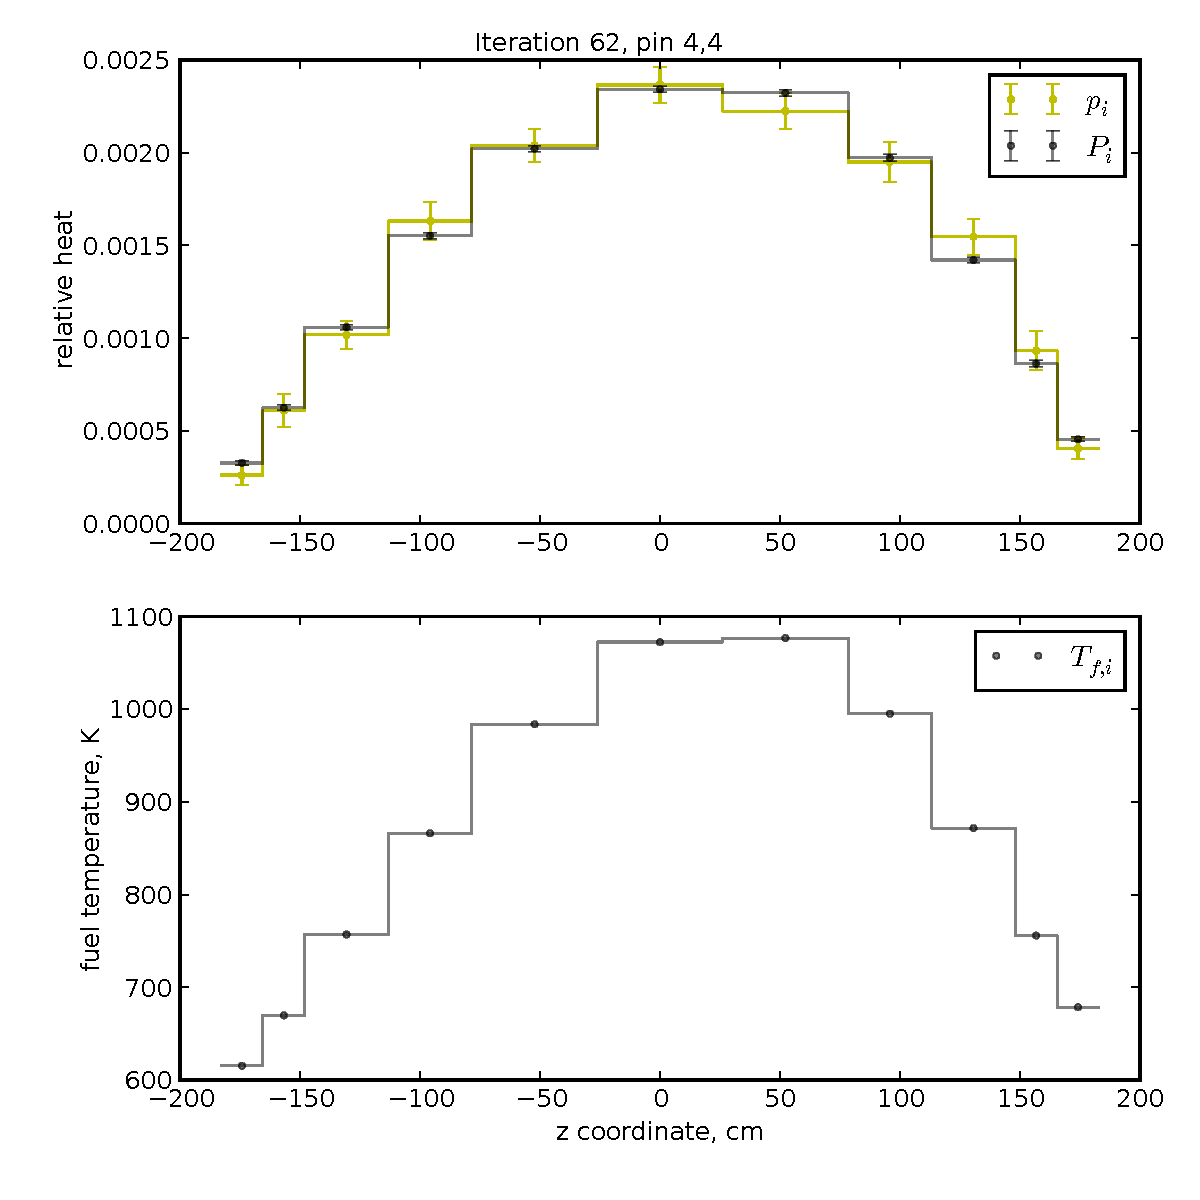
\includegraphics[trim=0 0 0 280,clip=true,width=0.8\textwidth]{pics/b_iteration_062_4_4.pdf}
\end{frame}

\begin{frame}\frametitle{Пример: результат совместного итеративного расчтеа}
    Картограмма температурных полей
            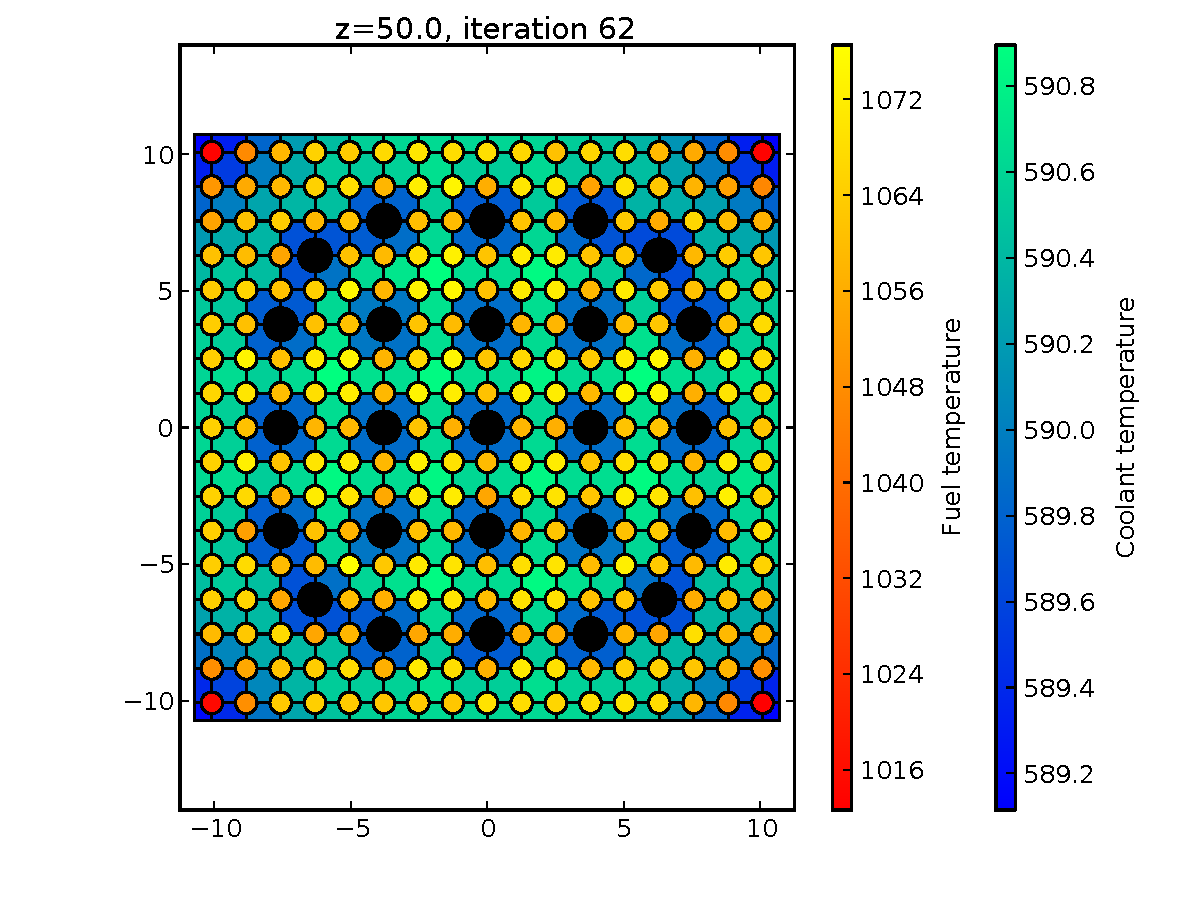
\includegraphics[width=0.7\textwidth]{pics/b_iteration_062_temp50_0.pdf}
\end{frame}


\section{Дальнейшая работа}
\begin{frame}\frametitle{Дальнейшая работа}

    \begin{block}{Сейчас}
        \begin{itemize}
            \item Интерфейс для SERPENT-2
            \item Применение на суперкомптьютере в Юлихе
            \item документация
        \end{itemize}
    \end{block}

    \begin{block}{В будущем}
        \begin{itemize}
            \item Переписать интерфейс к SCF
            \item отрисовка геометрии
            \item интерфейс к NMC 
        \end{itemize}
    \end{block}

    Есть желающие? anton.travleev@kit.edu


\end{frame}

\end{document}
